% !TEX TS-program = XeLaTeX
% use the following command: 
% all document files must be coded in UTF-8
\documentclass[english]{textolivre}
% for anonymous submission
%\documentclass[anonymous]{textolivre}
% to create HTML use 
%\documentclass{textolivre-html}
% See more information on the repository: https://github.com/leolca/textolivre

% Metadata
\begin{filecontents*}[overwrite]{article.xmpdata}
    \Title{Analysis of a Portuguese HEI teachers experience in the context of COVID-19}
    \Author{Elisabete Brito \sep Natália Gomes \sep Pedro Tadeu \sep Carlos Brigas}
    \Language{en}
    \Keywords{Teaching and learning methodologies \sep higher education \sep distance learning \sep collaborative tools }
    \Journaltitle{Texto Livre}
    \Journalnumber{1983-3652}
    \Volume{14}
    \Issue{2}
    \Firstpage{1}
    \Lastpage{12}
    \Doi{10.35699/1983-3652.2021.33579}

    \setRGBcolorprofile{sRGB_IEC61966-2-1_black_scaled.icc}
            {sRGB_IEC61966-2-1_black_scaled}
            {sRGB IEC61966 v2.1 with black scaling}
            {http://www.color.org}
\end{filecontents*}

% used to create dummy text for the template file
\definecolor{dark-gray}{gray}{0.35} % color used to display dummy texts
\usepackage{lipsum}
\SetLipsumParListSurrounders{\colorlet{oldcolor}{.}\color{dark-gray}}{\color{oldcolor}}

% used here only to provide the XeLaTeX and BibTeX logos
\usepackage{hologo}

% used in this example to provide source code environment
%\crefname{lstlisting}{lista}{listas}
%\Crefname{lstlisting}{Lista}{Listas}
%\usepackage{listings}
%\renewcommand\lstlistingname{Lista}
%\lstset{language=bash,
        breaklines=true,
        basicstyle=\linespread{1}\small\ttfamily,
        numbers=none,xleftmargin=0.5cm,
        frame=none,
        framexleftmargin=0.5em,
        framexrightmargin=0.5em,
        showstringspaces=false,
        upquote=true,
        commentstyle=\color{gray},
        literate=%
           {á}{{\'a}}1 {é}{{\'e}}1 {í}{{\'i}}1 {ó}{{\'o}}1 {ú}{{\'u}}1 
           {à}{{\`a}}1 {è}{{\`e}}1 {ì}{{\`i}}1 {ò}{{\`o}}1 {ù}{{\`u}}1
           {ã}{{\~a}}1 {ẽ}{{\~e}}1 {ĩ}{{\~i}}1 {õ}{{\~o}}1 {ũ}{{\~u}}1
           {â}{{\^a}}1 {ê}{{\^e}}1 {î}{{\^i}}1 {ô}{{\^o}}1 {û}{{\^u}}1
           {ä}{{\"a}}1 {ë}{{\"e}}1 {ï}{{\"i}}1 {ö}{{\"o}}1 {ü}{{\"u}}1
           {Á}{{\'A}}1 {É}{{\'E}}1 {Í}{{\'I}}1 {Ó}{{\'O}}1 {Ú}{{\'U}}1
           {À}{{\`A}}1 {È}{{\`E}}1 {Ì}{{\`I}}1 {Ò}{{\`O}}1 {Ù}{{\`U}}1
           {Ã}{{\~A}}1 {Ẽ}{{\~E}}1 {Ũ}{{\~u}}1 {Õ}{{\~O}}1 {Ũ}{{\~U}}1
           {Â}{{\^A}}1 {Ê}{{\^E}}1 {Î}{{\^I}}1 {Ô}{{\^O}}1 {Û}{{\^U}}1
           {Ä}{{\"A}}1 {Ë}{{\"E}}1 {Ï}{{\"I}}1 {Ö}{{\"O}}1 {Ü}{{\"U}}1
           {ç}{{\c{c}}}1 {Ç}{{\c{C}}}1
}


\journalname{Texto Livre}
\thevolume{14}
\thenumber{2}
\theyear{2021}
\receiveddate{\DTMdisplaydate{2020}{12}{11}{-1}} % YYYY MM DD
\accepteddate{\DTMdisplaydate{2021}{02}{28}{-1}}
\publisheddate{\DTMdisplaydate{2021}{06}{22}{-1}}
% Corresponding author
\corrauthor{Elisabete Brito}
% DOI
\articledoi{10.35699/1983-3652.2021.33579}
% list of available sesscions in the journal: articles, dossier, reports, essays, reviews, interviews, editorial
\articlesessionname{dossier}
% Abbreviated author list for the running footer
\runningauthor{Brito et al.}
\editorname{Anna Izabella M. Pereira} 

\title{Analysis of a Portuguese HEI teachers experience in the context of COVID-19}
\othertitle{Análise da experiência de professores do ensino superior português no contexto da COVID-19}
% if there is a third language title, add here:
%\othertitle{Artikelvorlage zur Einreichung beim Texto Livre Journal}

\author[1]{Elisabete Brito \orcid{0000-0001-9568-6532} \thanks{Email: \url{beta@ipg.pt}}}
\author[2]{Natália Gomes \orcid{0000-0002-1487-007X} \thanks{Email: \url{ngomes@ipg.pt}}}
\author[1]{Pedro Tadeu \orcid{0000-0002-0698-400X} \thanks{Email: \url{ptadeu@ipg.pt}}}
\author[1]{Carlos Brigas \orcid{0000-0003-2369-9427} \thanks{Email: \url{brigas@ipg.pt}}}

\affil[1]{Instituto Politécnico da Guarda, Escola Superior de Educação, Comunicação e Desporto - Unidade de Investigação para o Desenvolvimento do Interior, CI\&DEI - Centro de Estudos em Educação e Inovação, Guarda, Portugal.}
\affil[2]{Instituto Politécnico da Guarda, Escola Superior de Tecnologia e Gestão - Unidade de Investigação para o Desenvolvimento do Interior, CI\&DEI - Centro de Estudos em Educação e Inovação, Guarda, Portugal.}

\addbibresource{article.bib}
% use biber instead of bibtex
% $ biber tl-article-template

% set language of the article
\setdefaultlanguage{english}
\setotherlanguage{portuguese}

% for spanish, use:
%\setdefaultlanguage{spanish}
%\gappto\captionsspanish{\renewcommand{\tablename}{Tabla}} % use 'Tabla' instead of 'Cuadro'
%\AfterEndPreamble{\crefname{table}{tabla}{tablas}\Crefname{table}{Tabla}{Tablas}}

% for languages that use special fonts, you must provide the typeface that will be used
% \setotherlanguage{arabic}
% \newfontfamily\arabicfont[Script=Arabic]{Amiri}
% \newfontfamily\arabicfontsf[Script=Arabic]{Amiri}
% \newfontfamily\arabicfonttt[Script=Arabic]{Amiri}
%
% in the article, to add arabic text use: \textlang{arabic}{ ... }

% to use emoticons in your manuscript
% https://stackoverflow.com/questions/190145/how-to-insert-emoticons-in-latex/57076064
% using font Symbola, which has full support
% the font may be downloaded at:
% https://dn-works.com/ufas/
% add to preamble:
% \newfontfamily\Symbola{Symbola}
% in the text use:
% {\Symbola }

% reference itens in a descriptive list using their labels instead of numbers
% insert the code below in the preambule:
\makeatletter
\let\orgdescriptionlabel\descriptionlabel
\renewcommand*{\descriptionlabel}[1]{%
  \let\orglabel\label
  \let\label\@gobble
  \phantomsection
  \edef\@currentlabel{#1\unskip}%
  \let\label\orglabel
  \orgdescriptionlabel{#1}%
}
\makeatother
%
% in your document, use as illustraded here:
%\begin{description}
%  \item[first\label{itm1}] this is only an example;
%  % ...  add more items
%\end{description}
 

% custom epigraph - BEGIN 
%%% https://tex.stackexchange.com/questions/193178/specific-epigraph-style
\usepackage{epigraph}
\renewcommand\textflush{flushright}
\makeatletter
\newlength\epitextskip
\pretocmd{\@epitext}{\em}{}{}
\apptocmd{\@epitext}{\em}{}{}
\patchcmd{\epigraph}{\@epitext{#1}\\}{\@epitext{#1}\\[\epitextskip]}{}{}
\makeatother
\setlength\epigraphrule{0pt}
\setlength\epitextskip{0.5ex}
\setlength\epigraphwidth{.7\textwidth}
% custom epigraph - END


% if you use multirows in a table, include the multirow package
\usepackage{multirow}

% add line numbers for submission
%\usepackage{lineno}
%\linenumbers

\begin{document}
\maketitle

\begin{polyabstract}
\begin{abstract}
The current context of the pandemic crisis has led to unexpected educational changes. It has forced the institutions to rapidly adapt their teaching and learning methodologies in all areas, especially in higher education. This atypical situation, has given rise to numerous reflections on the ability of institutions to adapt to this new paradigm. This research aims to understand how the Portuguese Higher Education Institution (Polytechnic of Guarda) teachers have adjusted their teaching and learning process to distance learning. We constructed a quantitative investigation with a survey applied to the population, consisting of 158 individuals, achieving 102 valid answers, 65\% of the population. The results show that despite the initial doubts and concerns at the beginning of the process, there was always a substantial increase in work volume. There was a rapid adaptation to new teaching and learning methodologies in COVID-19 time. Overall, most of the inquiries considered this distance learning experience to be very positive.


\keywords{Teaching and learning methodologies \sep higher education \sep distance learning \sep collaborative tools }
\end{abstract}

\begin{portuguese}
\begin{abstract}
O contexto atual da crise pandémica levou a mudanças educacionais inesperadas. Obrigou as instituições a adaptar rapidamente as suas metodologias de ensino e aprendizagem em todas as áreas, especialmente no ensino superior. Esta situação, atípica, deu origem a inúmeras reflexões sobre a capacidade das instituições de se adaptarem a este novo paradigma. Esta pesquisa tem como objetivo entender como os professores de uma Instituição de Ensino Superior (Instituto Politécnico da Guarda) ajustaram o seu processo de ensino e aprendizagem à situação de ensino a distância. Foi construída uma investigação quantitativa com um levantamento aplicado à população, sendo esta composta por 158 elementos, alcançando 102 respostas válidas, 65\% da população. Os resultados mostram que, apesar das dúvidas e preocupações no início do processo, significando sempre um aumento substancial no volume de trabalho, houve uma rápida adaptação às novas metodologias de ensino e aprendizagem neste período de COVID-19. No geral, a maioria dos inquiridos considerou esta experiência de ensino a distância muito positiva.


\keywords{Metodologias de ensino e aprendizagem \sep ensino superior \sep ensino a distância; ferramentas colaborativas}
\end{abstract}
\end{portuguese}

% if there is another abstract, insert it here using the same scheme
\end{polyabstract}


\section{Introduction}\label{sec-intro}
In the current globalized knowledge society of constant scientific, technical innovation and technology, higher education institutions (HEIs) should consider distance learning (\emph{E@D - Ensino a distância}) as a fundamental factor in its strategic management policy. The HEI should reflect on its form of integration to empower students with essential competencies for the 21st century \cite{rodrigues2015}. Thus, the use of technologies should be thought of to make the teaching-learning process more efficient and effective, aiming that learning happens and is meaningful \cite{konrath2009}.

The Portuguese HEIs have shown concerns about incorporating new teaching methods compared to traditional methodology (face-to-face teaching). This happens through the implementation of several processes. Among these, we could state the following: Learning Management Systems (LMS) platforms; the creation of Massive Open Online Course (MOOC) courses; the design of courses in blended learning mode (b-learning) and by mobile learning (m-learning). These social learning or learning models are characterized by the ubiquity of collaborative systems and tools \cite{oliveira2015}.

Several studies show the advantages associated with this type of education, which enables all those involved (educational institutions, students and teachers) to obtain different benefits that contribute to supporting and increasing the effectiveness and success of educational systems \cite{alsabawy2016, mattar2020}.

During the Covid-19 pandemic, the \emph{E@D} emerged as the obligatory and necessary alternative to meet the pressing needs of a primarily unprepared educational community, but which quickly had to adapt to this reality in spaces and times different from face-to-face reality.

\section{Contextualization}
For public health reasons, in the COVID-19 pandemic, the world and the country stopped, schools closed. According to a study published in the spring of 2020, more than 1.2 billion children have had their classroom teaching activity suspended, altering teaching methods and developing and trying to adapt to \emph{E@D} in record time. This reality also extended to higher education, which, in Portugal, was until then mostly face-to-face. This had to be rethought and draw in new ways, had to reinvent itself to give immediate answers to a reality that needs a time of mise en place to respond to the demands of quality teaching.

The same study asks whether, effectively, after the pandemic, this education system will remain and ultimately be part of the educational strategy of all countries. It is essential to mention that before COVID-19, there was already, on the part of educational institutions, considerable growth in the introduction and use of digital technologies, with an investment in \emph{E@D} expected to exceed \$350 billion in 2025 \cite{li2020}. However, it should be noted that the implementation of this teaching-learning system has many socio-economic constraints, particularly in underdeveloped countries, due to the lack of an effective information society.

Thus, it is essential to reflect on the innovations that study on \emph{E@D} present, as well as on the methodologies and good practices of teachers, which allow making this teaching an effective learning environment and a competitive advantage for institutions \cite{mcgill2014, ilin2017}.

\section{Skills and role of the teacher in the \emph{E@D}}
The process of \emph{E@D} is not as simple as is sometimes stated, often denoting great ignorance and even some counter-information concerning this practice. It is not difficult to hear, wrongly, in some media and social networks that the process to take place is needed only by a teacher and the use of any technology. The growing diversity of platforms, the lack of knowledge of their use in creative, innovative and methodologically student-centred approaches, the absence or scarcity of digital skills on the part of teachers and students, the lack of strategies about the \emph{E@D} modality hinders not only the process but also its increasing use with quality, in institutions.

In the construction of online learning communities, increasingly present, one of the most critical aspects is student-centred learning, based on the premise that knowledge and relationships between participants are developing through the established interactions \cite{martinho2014}. In this line of thinking, knowledge about students is obtained and deepened in the same proportion that the collaborative learning process is developed and improved \cite{anderson2008, garrison2008, palloff2007}, to make students' teaching and learn more effectively, and the teacher's figure and understanding of his multiple roles in cyberculture times are fundamental: trainer, director of teaching materials, researcher, mediator and advisor \cite{bruno2010}.

\textcite{zwaneveld2007} argue that most ICT competencies for teachers are four: Individual media-competencies; critical media-competencies; lifelong learning competence; and Supervising learning process. Teachers must assume a multidimensional role and are urged to integrate a range of different and numerous competencies. According to \textcite{wake2007}, using ICT and new approaches to teaching and learning boost the foundation of two new areas of action: academic as a mentor and as an orchestrator.

The process of distance learning, as regards teaching, necessarily consider that the design, development, and assessment of virtual education introduce features and require specific teaching tasks \cite{major2010, spector2007}.

The role of the teacher is reinforced in \emph{E@D} environments since it requires more excellent monitoring, the use of motivation techniques and the use of more proactive methodologies. The teacher should thus be a facilitator of the process, promoting the use of virtual environments, collaborative tools and teaching processes directed to techniques and new methodologies \cite{dunlap2008, amitg2015}, of which can be examples of the following ones:

\begin{itemize}
    \item flipped learning;
    \item problem-based learning;
    \item gamification learning;
    \item creation of individual work plans;
    \item management of synchronous and asynchronous classes;
    \item making or reusing explanatory videos;
    \item conducting collaborative activities;
    \item diversification of resources and tools;
    \item ensuring more effective communication and feedback.
\end{itemize}

In this context, and due to the importance to understand advantages, disadvantages and potential and successful methodologies, this study aimed to systematically analyze the implementation level for e-learning (\emph{E@D}) in higher education system education from the Guarda Polytechnic Institute (IPG) in Portugal, during the COVID-19 pandemic.

\section{Methods}
The survey's target group consisted of professors teaching on the four schools of IPG in the city of Guarda and Seia, Portugal: School of Education, Communication and Sport; School of Technology and Management; School of Tourism and Hospitality Management and the School of Health Sciences. An item-based questionnaire was constructed based on a literature search. The items were grouped into the following three main areas:

\begin{itemize}
    \item General information about the demographic profile of the participants;
    \item Information about expectative, methodologies and platforms used in \emph{E@D};
    \item Information about personal measurement data working on \emph{E@D}.
\end{itemize}

The initial questionnaire was validated through a peer review approach online according to the pre-test method during the spring semester 2019/20. Peer reviewers (n = 4) were professors expert on e-learning education and ICT use within education environments. The returned comments were collected, and the questionnaire adapted accordingly to the suggestions made.

The final questionnaire for this study contained 27 items and was delivered to all professors teaching in the four schools. Access to the questionnaire was provided by an invitation email link supplied by Google Forms. The survey started in June 2020 and the data collection ended in September 2020. The analysis was undertaken using the SPSS 23 program. 

\section{Results}
In this section, we present the results obtained with the questionnaire. The first table (\Cref{tab1}) shows a characterization of the population of this study.  

\begin{table}[htpb]
\caption{Sociodemographic characterization}
\label{tab1}
\centering
\small
\begin{tabular}{p{0.15\textwidth}p{0.35\textwidth}p{0.08\textwidth}p{0.08\textwidth}}
\toprule 
\multicolumn{2}{c}{Variables} & N & \%
\\
\midrule
\arrayrulecolor[gray]{.7}
\multirow{3}{*}{Gender} & Male & 53 & 52,5\%
\\
%\cmidrule{2-4}
& Female & 48 & 47,5\%
\\
%\cmidrule{2-4}
& Total & 101 & 100\%
\\
\arrayrulecolor{black}
\midrule
\arrayrulecolor[gray]{.7}
\multirow{6}{=}{Age (years)} & Up to 45 years & 24 & 23,8\%
\\
%\cmidrule{2-4}
& From 46 to 50 years & 9 & 18,8\%
\\
%\cmidrule{2-4}
& From 51 to 55 years & 39 & 38,6\%
\\
%\cmidrule{2-4}
& More than 55 years & 19 & 18,8\%
\\
%\cmidrule{2-4}
& Total & 101 & 100%
\\
%\cmidrule{2-4}
& \multicolumn{3}{c}{Minimum=34; Maximum=64; Mean=50.53; Standard deviation=6.52}
\\
\arrayrulecolor{black}
\midrule
\arrayrulecolor[gray]{.7}
\multirow{5}{=}{Educational qualifications} & Degree & 4 & 4,0\%
\\
%\cmidrule{2-4}
& Master & 17 & 16,8\%
\\
%\cmidrule{2-4}
& PhD & 69 & 68,3\%
\\
%\cmidrule{2-4}
& Expert & 11 & 10,9\%
\\
%\cmidrule{2-4}
& Total & 101 & 100\%
\\
\arrayrulecolor{black}
\midrule
\arrayrulecolor[gray]{.7}
\multirow{5}{=}{School in IPG} & Superior School of Education, Communication and Sport \newline 
ESECD & 30 & 29,7\%
\\
%\cmidrule{2-4}
& Superior School of Technology and Management \newline
ESTG & 49 & 48,5\%
\\
%\cmidrule{2-4}
& Superior School of Health Sciences \newline
ESS & 13 & 12,9\%
\\
%\cmidrule{2-4}
& School of Tourism and Hospitality Management \newline
ESTH & 9 & 8,9\%
\\
%\cmidrule{2-4}
& Total & 101 & 100\%
\\
\arrayrulecolor{black}
\bottomrule
\end{tabular}
\centering
\source{own elaboration.}
\end{table}

There is an evident division regarding gender among professors (52,5\% male and 47,5\% female), regarding the age groups, the group between 51 and 55 years (38,6\%) overlap the other groups. The same happens with the qualifications; the group of persons that have PhD. is very significate in the institution (68,3\%). Schools are divided following a proportional dimension, with the most significant number of professors in ESTG (48,5\%) and the smallest in ESTH (8,9\%). 

The following table (\Cref{tab2}) shows the experience of taught and trained in the \emph{E@D} system.

\begin{table}[htpb]
\caption{Experience \emph{E@D}}
\label{tab2}
\centering
\small
\begin{tabular}{p{0.4\textwidth}p{0.2\textwidth}p{0.1\textwidth}p{0.1\textwidth}}
\toprule
\arrayrulecolor[gray]{.7}
\multirow{3}{*}{Throughout his career taught in \emph{E@D}} & Yes & 40 & 39,6\%
\\
%\cmidrule{2-4}
& No & 61 & 60,4\%
\\
%\cmidrule{2-4}
& Total & 101 & 100\%
\\
\arrayrulecolor{black}
\midrule
\arrayrulecolor[gray]{.7}
\multirow{3}{*}{Have you ever trained in \emph{E@D}} & Yes & 45 & 44,6\%
\\ 
%\cmidrule{2-4}
& No & 56 & 55,4\%
\\
%\cmidrule{2-4}
& Total & 101 & 100\%
\\
\arrayrulecolor{black}
\bottomrule
\end{tabular}
\centering
\source{own elaboration.}
\end{table}

Professors who have taught, or have trained in \emph{E@D}, are less than those who never had this type of experience, showing that most professors don't have experience in both situations.

\begin{figure}[htbp]
 \centering
 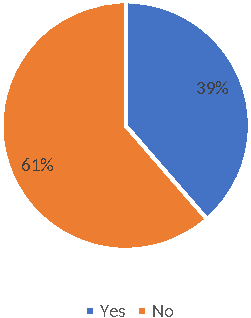
\includegraphics[width=0.35\textwidth]{Fig_001.pdf}
 \caption{ICT equipment bought}
 \label{fig1}
 \source{own elaboration.}
\end{figure}

There was an evident improvement of conditions at home to achieve the goal of \emph{E@D} classes, and we have 61\% of the professors that have brought new computer, or similar equipment, to deal with the process, as we see in Graph \ref{fig1}.

\begin{figure}[htbp]
 \centering
 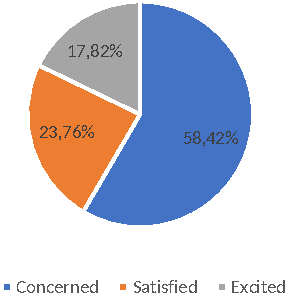
\includegraphics[width=0.35\textwidth]{Fig_002.pdf}
 \caption{Feeling at the beginning of the process about E@D}
 \label{fig2}
 \source{own elaboration.}
\end{figure}

Regarding the process, and before starting, most of the professors are very concerned with the process of \emph{E@D} (58,42\%), as we see in Graph \ref{fig2}. 

The following table (\Cref{tab3}) gives some details regarding the essential options to achieve the objectives in the different syllabus of the institution degrees.

\begin{table}[htpb]
\caption{Experience \emph{E@D}}
\label{tab3}
\small
\centering
\begin{tabular}{p{0.4\textwidth}p{0.06\textwidth}p{0.2\textwidth}p{0.2\textwidth}}
\toprule
& \multicolumn{2}{c}{Answers} & \multirow{2}{*}{\% (total respondents)}
\\
\cmidrule{2-3}
& N & \% (total responses) & 
\\
\midrule
\arrayrulecolor[gray]{.7}
Learn how the video conferencing platform would work & 49 & 16,3\% & 48,5\%
\\
%\midrule
Develop new methodologies that promote a more active role of students & 52 & 17,3\% & 51,5\%
\\
%\midrule
Change curriculum planning & 28 & 9,3\% & 27,7\%
\\
%\midrule
Change evaluation methods & 41 & 13,6\% & 40,6\%
\\
%\midrule
Establish new approaches during the presentations/online classes & 52 & 17,3\% & 51,5\%
\\
%\midrule
Define new practical exercises & 40 & 13,3\% & 39,6\%
\\
%\midrule
Define new bibliography and/or complementary information on the Internet & 12 & 4,0\% & 11,9\%
\\
%\midrule
Search for information so that students can complement their study through the Flipped Learning methodology & 16 & 5,3\% & 15,8\%
\\
%\midrule
Make videos explaining the story & 11 & 3,7\% & 10,9\%
\\
%\midrule
Total & 301 & 100,0\% & 
\\
\arrayrulecolor{black}
\bottomrule
\end{tabular}
\centering
\source{own elaboration.}
\end{table}

In the last question, the respondents can choose a maximum of three option among the different suggestions. The main options choose, \emph{Develop new methodologies that promote a more active role of students} (17,3\%) and \emph{Establish new approaches during the presentations/online classes} (17,3\%). On the other hand, the options that were not chosen so often were \emph{Make videos explaining the story} (3,7\%) and \emph{Define new bibliography and/or complementary information on the Internet} (4,0\%).

The following table (\Cref{tab4}) defines the perspective of professors before starting the process concerning the traditional education process versus the new \emph{E@D} using a Likert scale (1- Totally disagree; 2- Disagree; 3- Neither agree nor disagree; 4- I agree; 5- Totally Agree).

\begin{table}[htpb]
\caption{Characteristics of the teacher's perspective regarding \emph{traditional education} versus \emph{E@D} in pandemic}
\label{tab4}
\centering
\small
\begin{tabular}{p{0.55\textwidth}p{0.1\textwidth}p{0.1\textwidth}p{0.1\textwidth}}
\toprule
Items & Average & Standard deviation & Median
\\
\midrule
\arrayrulecolor[gray]{.7}
I easily adapted to this new methodology & 4,11 & 0,85 & 4,00
\\
%\midrule
Easily adapted to the use of new platforms and collaborative tools & 4,18 & 0,78 & 4,00
\\
%\midrule
I've spent more time planning and preparing classes & 4,62 & 0,63 & 5,00
\\
%\midrule
I developed teaching methodologies that promoted the active role of students in the search for new learning & 4,04 & 0,81 & 4,00
\\
%\midrule
Promoting the development of the competencies areas of the students' profile & 3,91 & 0,83 & 4,00
\\
%\midrule
I reformed the way I taught classes & 4,24 & 0,68 & 4,00
\\
%\midrule
I've been adhering to the teaching materials & 4,24 & 0,74 & 4,00	\\
%\midrule
I've set the evaluation parameters & 4,19 & 0,96 & 4,00
\\
%\midrule
I have changed the teaching and learning process to promote the greater autonomy of students & 4,04 & 0,86 & 4,00
\\
%\midrule
I have changed the teaching and learning process to be more dynamic and interactive & 4,05 & 0,74 & 4,00
\\
%\midrule
I have changed the teaching and learning process so that most classes can take place asynchronously & 2,47 & 1,33 & 2,00
\\
%\midrule
I encouraged the establishment of regular communications & 4,37 & 0,73 & 5,00
\\
%\midrule
I've deferred more time to clarify doubts & 4,12 & 0,85 & 4,00	
\\
\arrayrulecolor{black}
\bottomrule
\end{tabular}
\centering
\source{own elaboration.}
\notes{Cronbach's Alpha = 0.786}
\end{table}

The previous table (\Cref{tab4}) indicates that the professors choose \emph{I've spent more time planning and preparing classes} most of the times with an average of 4,62 and a median of 5, giving a clear signal that most of them agree with this statement. Contrary to the answer, \emph{I have the teaching and learning process so that most classes can take place asynchronously}, that collect a mean of 2,47 and a median of 2. A large number of professors was not choosing the asynchronous process is preferable.

The following graph (\ref{fig3}) compares the professor expectations before and after the process.

\begin{figure}[htbp]
 \centering
 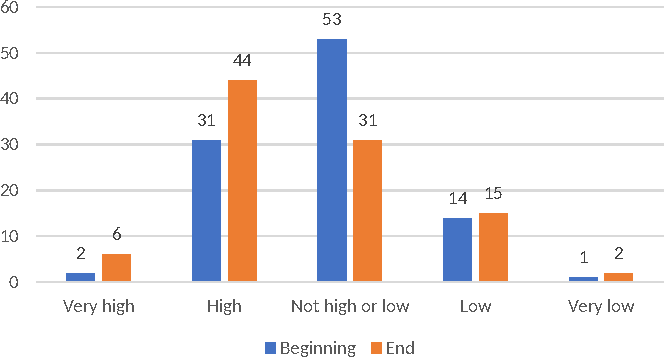
\includegraphics[width=0.75\textwidth]{Fig_003.pdf}
 \caption{Teacher expectation level (before and after)}
 \label{fig3}
 \source{own elaboration.}
\end{figure}

From the graphic, we observe that the professors who have low and very low expectations at the beginning maintained this opinion. The professors that didn't have either low or high expectations (\emph{not high or low}) have changed their opinion after going through the process by raising the \emph{very high} and the \emph{high values} of the answers. 

The following graphic (\ref{fig4}) show the results of the professor's expectations regarding the students.

\begin{figure}[htbp]
 \centering
 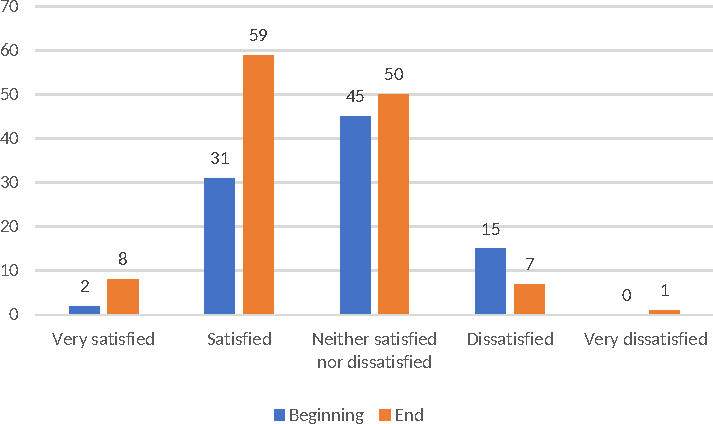
\includegraphics[width=0.75\textwidth]{Fig_004.pdf}
 \caption{Teacher perception of student satisfaction (before and after)}
 \label{fig4}
 \source{own elaboration.}
\end{figure}

There was an evident increase of the \emph{very satisfied} and \emph{satisfied} options when comparing the beginning and end of the process expectations regarding the students in the professors' point of view. 

The following graphic (\ref{fig5}) shows professors' perception regarding the necessary competencies that students have to develop a good autonomous work in the \emph{E@D} on the use of tools.

\begin{figure}[h!]
 \centering
 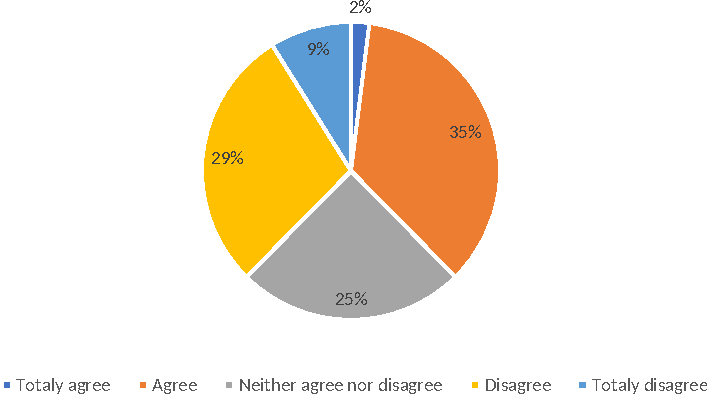
\includegraphics[width=0.8\textwidth]{Fig_005.pdf}
 \caption{Does the majority of students have the skills to develop an autonomous, responsible and critically study in \emph{E@D}?}
 \label{fig5}
 \source{own elaboration.}
\end{figure}

There isn't a clear vision from the answers giving by the professors; 38\% \emph{disagree} and \emph{totally disagree}, while 37\% \emph{agree} and \emph{totally agree}. This opposite vision could be explained by the different types of degrees and syllabus existing inside the institution. 

Graph \ref{fig6} shows the number of daily hours of work in front of a computer.

\begin{figure}[h!]
 \centering
 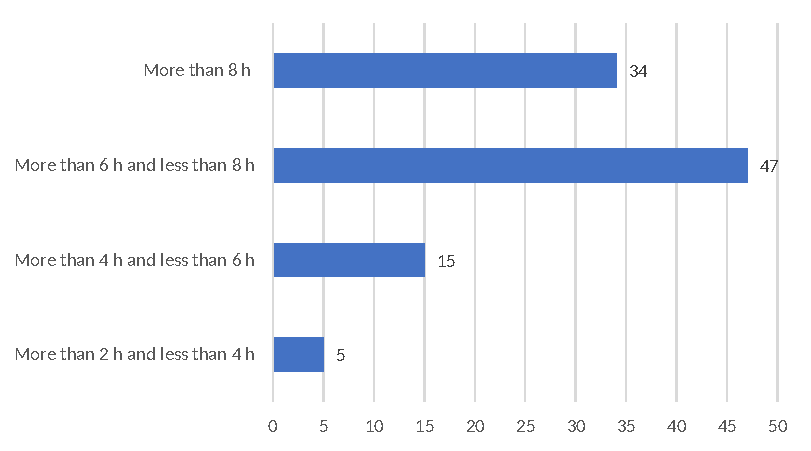
\includegraphics[width=0.85\textwidth]{Fig_006.pdf}
 \caption{Number of hours daily working in front of the computer}
 \label{fig6}
 \source{own elaboration.}
\end{figure}

Almost 48\% of the professors spend between 6 hours and 8 hours per day, and a significant number, 35\%, spend more than 8 hours in front of a computer. This includes the regular synchronous classes and all the necessary preparation.

The following figure (\ref{fig7}) shows the desire of the professors regarding the methodology that could be applied in the next year. 

\begin{figure}[htbp]
 \centering
 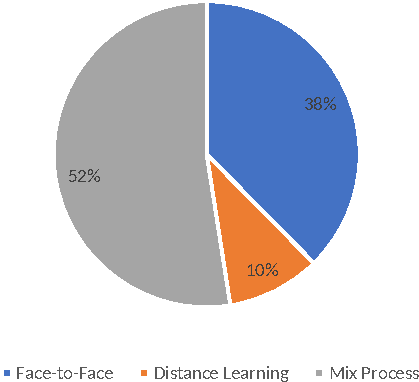
\includegraphics[width=0.4\textwidth]{Fig_007.pdf}
 \caption{What teaching methodology would you choose for 2020/2021.}
 \label{fig7}
 \source{own elaboration.}
\end{figure}

Most professors prefer a mixed process from the analyses, a b-learning methodology (52\%), while a small number (10\%) prefer the pure \emph{E@D}. It's interesting to notice that the process used for so long, the face-to-face, only enters in the preferences of 38\% of the professors.

\section{Conclusions}
In the context of the COVID-19 pandemic, the world and the country stopped, schools closed, due to the Covid-19 pandemic, the E@D emerged as the obligatory and necessary alternative to meet the pressing needs of a primarily unprepared educational community, but which quickly had to adapt to this reality, in spaces and times different from face-to-face reality. 

Students, teachers and all the intervenient in environment education altering teaching methods and trying to adapt methodologies, materials and IT tools to \emph{E@D}. 

The present study has the intention to draw the situation regarding de methodologies and digitally enhanced learning and teaching practice at the HEI Polytechnic of Guarda in Portugal.

With this study, we obtained results that allow us to understand how the teachers of a Higher Education Institution (Polytechnic of Guarda) have adapted their teaching-learning process to the situation of distance learning, their expectations.

The survey's target group consisted of all professors teaching at the four schools of IPG in Guarda and Seia, Portugal (School of Education, Communication and Sport; School of Technology and Management; School of Tourism and Hospitality Management and the School of Health Sciences). 

The results obtained with the questionnaire underline the following aspects:

\begin{itemize}
    \item The number of professors who have taught, or have trained in E@D, is less than those who never had this type of experience in teaching or training. This shows that most of the professors don't have experience in both situations.
    \item Most teachers purchased equipment that would allow them to carry out all the tasks planned during the classes.
    \item The study also made it possible to verify that most teachers were not confident in adhering to the distance learning methodology.
    \item To achieving the objectives, teachers develop new methodologies that promote a more active role of students and establish new approaches during the presentations/online classes. This demonstrated that teachers spent more time preparing the lessons and materials.
    \item Teachers preferred to perform synchronous tasks instead of asynchronous tasks.
    \item Regarding the necessary competencies that students have, develop good autonomous work in the E@D on tools. In this case, isn't a clear vision from the answers giving by the professors
    \item When professors are asked about the methodology that could be applied in the following year, the results show us that most prefer a mixed process, b-learning methods, while a small number prefer the pure \emph{E@D}. Another interesting fact is that the approach being used for so long, face-to-face, only enter in the preferences of 38\% of the professors.
\end{itemize}

The results obtained through the application of surveys show a great capacity of teachers to adapt to this new reality despite the initial doubts and concerns at the beginning of the process. Other relevant aspects are the investment in the acquisition of hardware, the increase in work resulting from the need for more time for the preparation of classes, the adaptation of didactic materials, and reformulating the way they were taught. On the other hand, there was a quick adaptation to new teaching and learning methodologies, most of which considered this distance learning experience very positive.

Nevertheless, we can mention that despite this fast adaptability, teachers continue to prefer synchronous activities. In their perspective, in future situations, the use of b-learning models should be privileged.

Like it was stated in the \textcite{gaebel2021},

\begin{quote}
    Months of unvoluntary remote learning and teaching have brought a clear demonstration that all that is technically possible is not socially desirable. These, rather than questions of technology and more or less online or blended learning, are the issues that will have to drive the discussions on the transformation of higher education.
\end{quote}

So each institution must make a deep analysis of its structure, conditions, human resources, and the students. Studies like these could help the HEI achieve better results and adapt to new realities, either because we are inside the XXI century (the old future) or because pandemic situations turn upside down the old fashioned contexts that tend to appear more often.

\section*{Acknowledge}
This work is funded by National Funds through the FCT - Foundation for Science and Technology, I.P., within the scope of the project Refª UIDB/05507/2020. Furthermore we would like to thank the Centre for Studies in Education and Innovation (CI\&DEI) and the Polytechnic of Guarda for their support. 

%%%%%%%%%%%%%%%%%%%%%%%%%%%%%%%%%%%%%%%%%%%%%%%%%%%%%%%%%%%%%%%%%%%%%%%%%%%%%%%%%%%%%%%%%%%%%%%%%%%%%%%%%%%%%%%%%%%%%%%%%%%%%%%%%%%%%%%%%%%%%%%%%%%%%%%%%%%%%%%%%%%%%%%%%%%%%%%%%%%%%%%%%%%%%%%%%%%%%%%%%%%%%%%%%%%%%%%%%%%%%%%%%%%%%%%%%%%%%%%%%%%%%%%%%%%%%%%%%%%%%%%%%%%%%%%%%%%%%%%%%%%%%%%%%%%%%%%%%%%%%%%%%%%%%%%%%%%%%%%%%%%%%%%%%%%%%%%%%%%%%%%%%%%%%%%%%%%%%%%%%%%%%%%%%%%%%%%%%%%%%%%%%%%%%%%%%%%%%%%%%%%%%%%%%%%%%%%%%%%%%%%%%%%%%%%%%%%%%%%%%%%%%%%%%%%%%%%%%%%%%%%%%%%%%%%%%%%%%%%%%%%%%%%%%%%%%%%%%%%%%%555


\printbibliography\label{sec-bib}
% if the text is not in Portuguese, it might be necessary to use the code below instead to print the correct ABNT abbreviations [s.n.], [s.l.] 
%\begin{portuguese}
%\printbibliography[title={Bibliography}]
%\end{portuguese}

\end{document}
